\chapter{The Bootstrap}

\inputminted{python}{../code/bootstrap.py}

% 1
\begin{ex}
  \textit{Note: In the second printing of the book, there is a mistake in the
    data given in the table in Example 8.6. The last GPA entry should be 2.95
    instead of 3.96. We will solve the problem using the corrected data.}

  \inputminted{python}{../code/08-01.py}
  \inputminted{text}{../output/08-01.txt}
\end{ex}

\begin{ex}
  To be able to estimate the coverage of the three intervals, we have to know
  the true value of the statistical functional $T$. To that end, let
  $Y\sim N(0, 1)$ and $X=e^Y$, and note that then
  \begin{align*}
    \E{X^k}
     & =\E{\exp\left\{kY\right\}}                                 \\
     & =\frac{1}{\sqrt{2\pi}}\int_{-\infty}^\infty\!
    \exp\left\{-\frac{1}{2}y^2+ky\right\}\,\d{y}                  \\
     & =\exp\{k^2/2\}\frac{1}{\sqrt{2\pi}}\int_{-\infty}^\infty\!
    \exp\left\{-\frac{1}{2}(y-k)^2\right\}\,\d{y}                 \\
     & =\exp\{k^2/2\}.
  \end{align*}
  Thus,
  \begin{align*}
    \mu = \E{X}        & =\sqrt{e},               \\
    \E{X^2}           =e^2,
    \sigma^2 = \var{X} & =\E{X^2}-\E{X}^2=e(e-1), \\
    \E{X^3}            & =e^4\sqrt{e},
  \end{align*}
  and therefore
  \begin{align*}
    \E{\left(\frac{X-\mu}{\sigma}\right)^3}
     & =\frac{\E{X^3}-3\mu(\E{X^2} - \mu\E{X})-\mu^3}{\sigma^3} \\
     & =\frac{\E{X^3}-3\mu\sigma^2-\mu^3}{\sigma^3}             \\
     & =\frac{e\sqrt{e}(e-1)^2(e+2)}{e(e-1)\sqrt{e}\sqrt{e-1}}  \\
     & =(e+2)\sqrt{e-1}.
  \end{align*}

  \inputminted{python}{../code/08-02.py}
  \inputminted{text}{../output/08-02.txt}
\end{ex}

\begin{ex}~
  \inputminted{python}{../code/08-03.py}
  \inputminted{text}{../output/08-03.txt}
\end{ex}

\begin{ex}
  Note that there is a bijection between size $n$ multisets of $k$ distinct
  elements and strings of $k-1$ bars and $n$ stars since the bars partition such
  a string into $k$ pieces, each of which we can take to correspond to one of
  the distinct elements, and where we can take the number of stars inside that
  part to be the number of times that element is present in the multiset.
  Note that such strings are of length $n+k-1$ and are uniquely determined by
  the location of the stars. Hence, there are
  \[
    \binom{n+k-1}{n}
  \]
  such multisets.

  When bootstrapping from a sample of $n$ distinct observations, the distinct
  bootstrap samples correspond to size $n$ multisets of $n$ distinct elements.
  Hence, there are
  \[
    \binom{2n-1}{n}
  \]
  of them.
\end{ex}

% 5
\begin{ex}
  We have
  \begin{align*}
    \cE{\Xbar^*}{X_1,\ldots,X_n}
     & =\cE{\frac{1}{n}\sum_{i=1}^n X^*_i}{X_1,\ldots,X_n}   \\
     & =\frac{1}{n}\sum_{i=1}^n \cE{X^*_i}{X_1,\ldots,X_n}   \\
     & =\frac{1}{n}\sum_{i=1}^n\sum_{j=1}^n \P{X^*_i=X_j}X_j \\
     & =\frac{1}{n}\sum_{i=1}^n\sum_{j=1}^n \frac{1}{n}X_j   \\
     & =\Xbar,
  \end{align*}
  and therefore, by the law of total expectation,
  \[
    \E{\Xbar^*}
    =\E{\cE{\Xbar^*}{X_1,\ldots,X_n}}
    =\E{X_1}.
  \]

  Note that
  \begin{align*}
    \cVar{X_i^*}{X_1,\ldots,X_n}
     & =\cE{(X_i^*-\Xbar^*)^2}{X_1,\ldots,X_n} \\
     & =\sum_{j=1}^n\P{X_i^*=X_j}(X_j-\Xbar)^2 \\
     & =\sum_{j=1}^n\frac{(X_j-\Xbar)^2}{n},
  \end{align*}
  and that therefore
  \[
    \cVar{\Xbar^*}{X_1,\ldots,X_n}
    =\frac{n}{n^2}\cVar{X_i^*}{X_1,\ldots,X_n}
    =\frac{1}{n}\sum_{j=1}^n\frac{(X_j-\Xbar)^2}{n}.
  \]
  Therefore, by the law of total variance,
  \begin{align*}
    \var{\Xbar^*}
     & =\E{\cVar{\Xbar^*}{X_1,\ldots,X_n}}
    +\var{\cE{\Xbar^*}{X_1,\ldots,X_n}}               \\
     & = \E{\frac{n-1}{n^2}S^2} + \var{\overline{X}}  \\
     & =\frac{n-1}{n^2}\var{X_1}+\frac{1}{n}\var{X_1} \\
     & =\frac{2n-1}{n^2}\var{X_1}.
  \end{align*}
\end{ex}

\begin{ex}~
  \begin{enumerate}[(a)]
    \item
          Note that for $X\sim N(\mu, \sigma^2)$ and $Y=e^X$, we have
          \[
            f_Y(x)
            =\frac{\d}{\d{x}}\P{Y\leq x}
            =\frac{\d}{\d{x}}\P{X\leq \log{x}}
            = \frac{\d}{\d{x}}\Phi\left(\frac{\log{x}-\mu}{\sigma}\right)
            = \frac{1}{x\sigma}\phi\left(\frac{\log{x}-\mu}{\sigma}\right).
          \]
          Therefore, recalling that $\overline{X}_n\sim N(\mu, \sigma^2/n)$,
          it follows that
          \[
            f_{\widehat{\theta}}(x)
            =\frac{\sqrt{n}}{x\sqrt{2\pi}}\exp\left\{-\frac{n(\log{x}-5)^2}{2} \right\},
          \]
          and that therefore $\widehat{\theta}$ follows a log-normal
          distribution with $\mu=5$ and $\sigma^2=1/n$.

          \inputminted{python}{../code/08-06.py}
          \inputminted{text}{../output/08-06.txt}
    \item ~
          \begin{figure}[H]
            \centering
            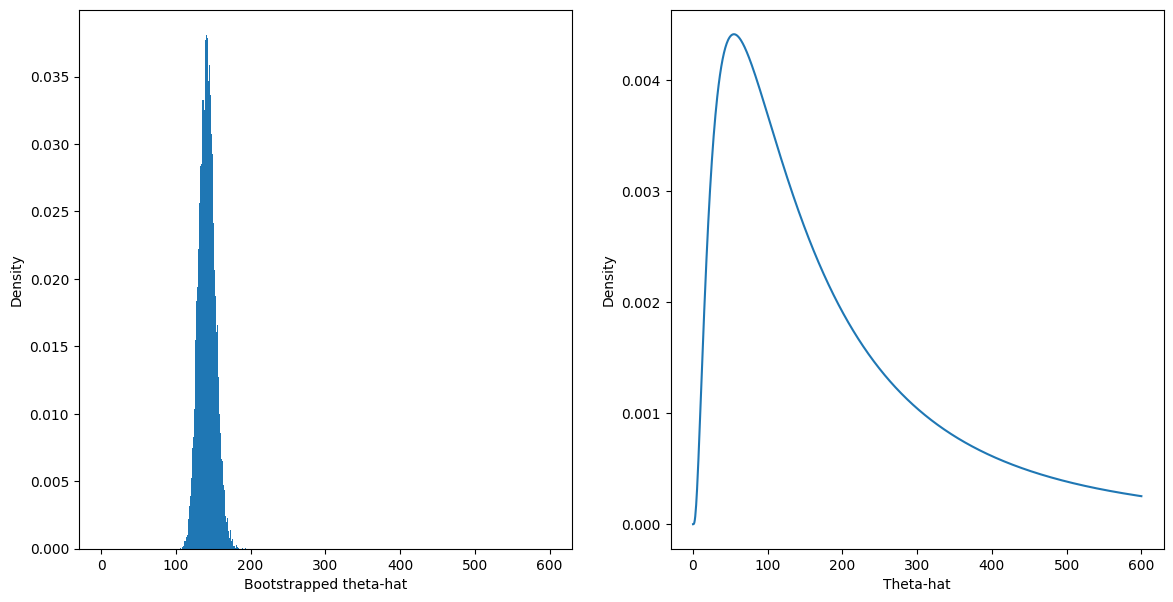
\includegraphics[scale=0.53]{../images/08-06}
            \caption{A comparison of a histogram of the bootstrap replications
              (left) and a plot of the true sampling distribution of
              $\widehat{\theta}$ (right). Note that the bootstrap underestimates
              the true variance of the sampling distribution, and fails to
              capture its skewness.}
          \end{figure}
  \end{enumerate}
\end{ex}

\begin{ex}~
  \begin{enumerate}[(a)]
    \item Note that
          \begin{align*}
            \P{\widehat{\theta}\leq x}
             & =\P{X_1\leq x,X_2\leq x,\ldots,X_n\leq x}      \\
             & =\P{X_1\leq x}\P{X_2\leq x}\cdots\P{X_n\leq x} \\
             & =(x/\theta)^n,
          \end{align*}
          and that therefore
          \[
            f_{\widehat{\theta}}(x)
            =\frac{\d}{\d{x}}\P{\widehat{\theta}\leq x}
            =n x^{n-1}/\theta^n.
          \]

          \inputminted{python}{../code/08-07.py}

          \begin{figure}[H]
            \centering
            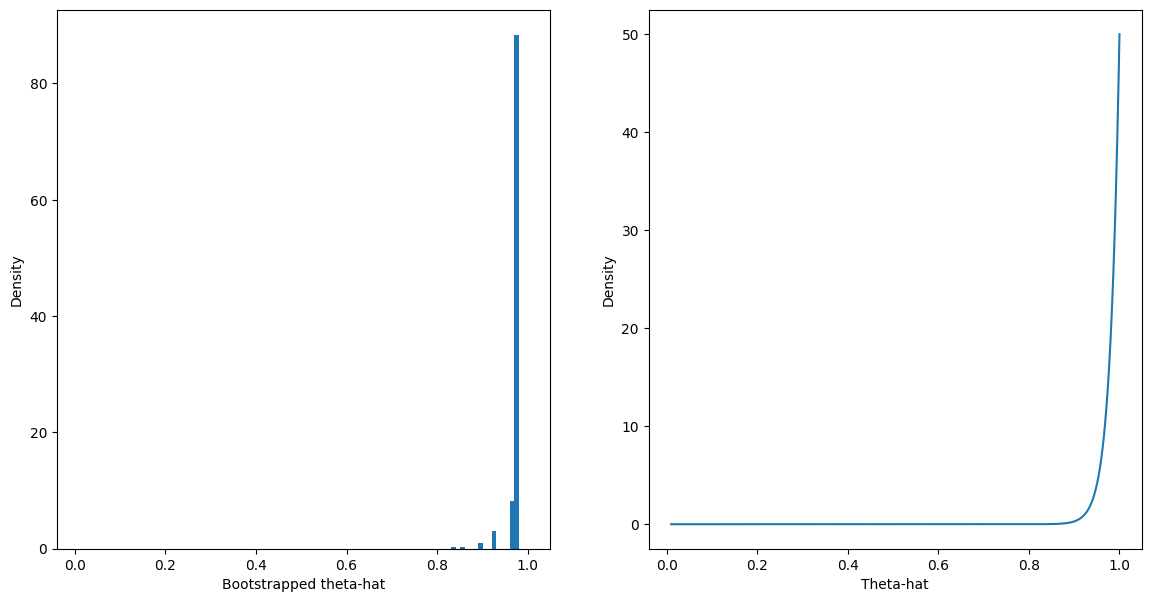
\includegraphics[scale=0.54]{../images/08-07}
            \caption{A comparison of a histogram of the bootstrap replications
              (left) and a plot of the true sampling distribution of
              $\widehat{\theta}$ (right).}
          \end{figure}
    \item Let $B$ be a random variable given by uniformly randomly sampling
          from $\{X_1,X_2,\ldots,X_n\}$, and let $B^n$ be a sample (with
          replacement) of $n$ elements. Then,
          \begin{align*}
            \P{\widehat{\theta}^*=\widehat{\theta}}
             & =\P{X_{(n)}\in B^n}              \\
             & =1-\P{X_{(n)}\not\in B^n}        \\
             & =1-(1-\P{B = X_{(n)}})^n         \\
             & =1-\left(1-\frac{1}{n}\right)^n,
          \end{align*}
          and therefore
          \[
            \lim_{n\to\infty}\P{\widehat{\theta}^*
              =\widehat{\theta}}
            =1-e^{-1}
            \approx 0.632.
          \]
          However, since $\widehat{\theta}$ has a continuous distribution, the
          probability that it takes on any particular value is $0$. Therefore,
          we cannot use the bootstrap to obtain an arbitrarily good
          approximation of $\widehat{\theta}$, no matter how many samples we
          use.
  \end{enumerate}
\end{ex}

\begin{ex}
  Let $T_1,\ldots,T_n$ be IID random variables with mean $0$. Let
  $S=T_1+\cdots+T_n$. Then
  \begin{align*}
    \E{S^2}
     & =\sum_{i=1}^n \E{T_i^2}
    =n\E{T_1^2},                                                                          \\
    \E{S^3}
     & =\sum_{i=1}^n \E{T_i^3}
    =n\E{T_1^3},                                                                          \\
    \E{S^4}
     & =\sum_{i=1}^n \E{T_i^4}+6\sum_{j=1}^n\sum_{\substack{k = j+1}}^n\E{T_j^2}\E{T_k^2}
    =n\E{T_1^4}+3n(n-1)\left[\E{T_1^2}\right]^2,
  \end{align*}
  since all terms in the multinomial expansion involving a factor of $\E{T_i}$
  are zero in expectation.

  Let $U=\sum_{i=1}^n X_i^*$, and let
  $Z=U-n\Xbar=\sum_{i=1}^n(X_i^*-\Xbar)=\sum_{i=1}^n Z_i$. We then have
  \begin{align*}
    \var{\left[\Xbar^*\right]^2}
     & =\var{\frac{U^2}{n^2}} \\
     & =\frac{1}{n^4}\left\{
    \E{U^4}
    +\E{U^2}^2
    \right\}                  \\
     & =\frac{1}{n^4}\bigg\{
    \left[\E{Z^4}
      +4\E{Z^3}(n\Xbar)
      +6\E{Z^2}(n\Xbar)^2
      +4\E{Z}(n\Xbar)^3
      +(n\Xbar)^4
      \right]                 \\
     & \qquad-\left[
      \E{Z^2}^2
      +4\E{Z^2}\E{Z}(n\Xbar)
      +4\E{Z}(n\Xbar)^3
      +2\E{Z^2}(n\Xbar)^2
      +(n\Xbar)^4
      \right]\bigg\}          \\
     & =\frac{1}{n^4}
    \left[\E{Z^4}
      +4\E{Z^3}(n\Xbar)
      +4\E{Z^2}(n\Xbar)^2
      -\E{Z^2}^2
      \right]                 \\
     & =\frac{1}{n^4}
    \left[
      n\E{Z_1^4}+3n(n-1)\E{Z_1^2}^2
      +4n^2\Xbar\E{Z_1^3}
      +4n^3\Xbar^2\E{Z_1^2}
      -n^2\E{Z_1^2}^2
      \right]                 \\
     & =
    \frac{4\Xbar^2\alphahat_2}{n}
    +\frac{4\Xbar\alphahat_3+2\alphahat_2^2}{n^2}
    +\frac{\alphahat_4-3\alphahat_2^2}{n^3}.
  \end{align*}
\end{ex}